\documentclass[border=.1cm]{standalone}

\usepackage{tikz}
\usepackage{times}
\usepackage{pgfplots}
\usepgflibrary{arrows}

\usepackage{siunitx}
\sisetup{
    detect-all = true,
    input-decimal-markers = {.},
    input-ignore = {,},
    inter-unit-product = \ensuremath{{}\cdot{}},
    multi-part-units = repeat,
    number-unit-product = \text{~},
    per-mode = fraction,
    separate-uncertainty = true,
}

\begin{document}

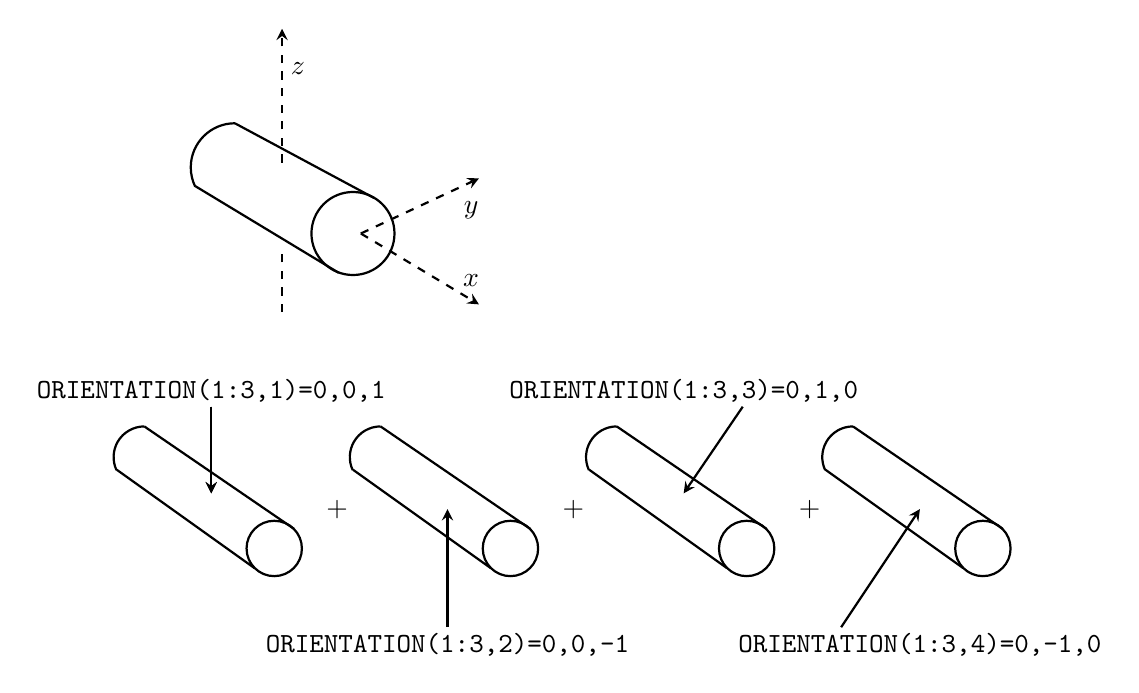
\begin{tikzpicture}

\draw [thick] (0,0) circle (10pt);
\draw[thick] (-.25,-.25) -- (-2,1);
\draw [thick] (.25,.25) -- (-1.65,1.55);
\draw [thick] (-1.65,1.55) arc ( 90: 205 :  .39cm);
\draw [-stealth, thick] (-.8,1.8) -- (-.8,.7);
\node at (-.8,2) {\tt ORIENTATION(1:3,1)=0,0,1};

\node at (.8,.5) {+};

\draw [thick] (3,0) circle (10pt);
\draw[thick] (2.75,-.25) -- (1,1);
\draw [thick] (3.25,.25) -- (1.35,1.55);
\draw [thick] (1.35,1.55) arc ( 90: 205 :  .39cm);
\draw [-stealth, thick] (2.2,-1) -- (2.2,.5);
\node at (2.2,-1.22) {\tt ORIENTATION(1:3,2)=0,0,-1};

\node at (3.8,.5) {+};

\draw [thick] (6,0) circle (10pt);
\draw[thick] (5.75,-.25) -- (4,1);
\draw [thick] (6.25,.25) -- (4.35,1.55);
\draw [thick] (4.35,1.55) arc ( 90: 205 :  .39cm);
\draw [-stealth, thick] (5.95,1.8) -- (5.2,.7);
\node at (5.2,2) {\tt ORIENTATION(1:3,3)=0,1,0};

\node at (6.8,.5) {+};

\draw [thick] (9,0) circle (10pt);
\draw[thick] (8.75,-.25) -- (7,1);
\draw [thick] (9.25,.25) -- (7.35,1.55);
\draw [thick] (7.35,1.55) arc ( 90: 205 :  .39cm);
\draw [-stealth, thick] (7.2,-1) -- (8.2,.5);
\node at (8.2,-1.22) {\tt ORIENTATION(1:3,4)=0,-1,0};

\draw [thick] (1,4) circle (15pt);
\draw[thick] (.82,3.5) -- (-1,4.6);
\draw [thick] (1.27,4.45) -- (-.5,5.4);
\draw [thick] (-.5,5.4) arc ( 90: 206 :  .56cm);
\draw [-stealth, thick] (-.8,1.8) -- (-.8,.7);

\draw[-stealth, dashed, thick] (1.1,4) -- (2.6,3.1);
\node at (2.5,3.4) {$x$};

\draw[-stealth, dashed, thick] (1.1,4) -- (2.6,4.7);
\node at (2.5,4.3) {$y$};

\draw[-stealth, dashed, thick] (.1,4.9) -- (.1,6.6);
\draw[ dashed, thick] (.1,3) -- (.1,3.84);
\node at (.3,6.1) {$z$};





\end{tikzpicture}

\end{document}
